Abbildung    \ref{fig:milestones}    beinhaltet     eine    \"Ubersicht    der
Meilensteine. Der  detaillierte Projektplan  ist in  Anhang \ref{app:psp}  auf
Seite \pageref{app:psp} zu finden.

%\begin{figure}[h!,width=\pageheight]
%\begin{figure}[h!]
%\begin{center}
%    %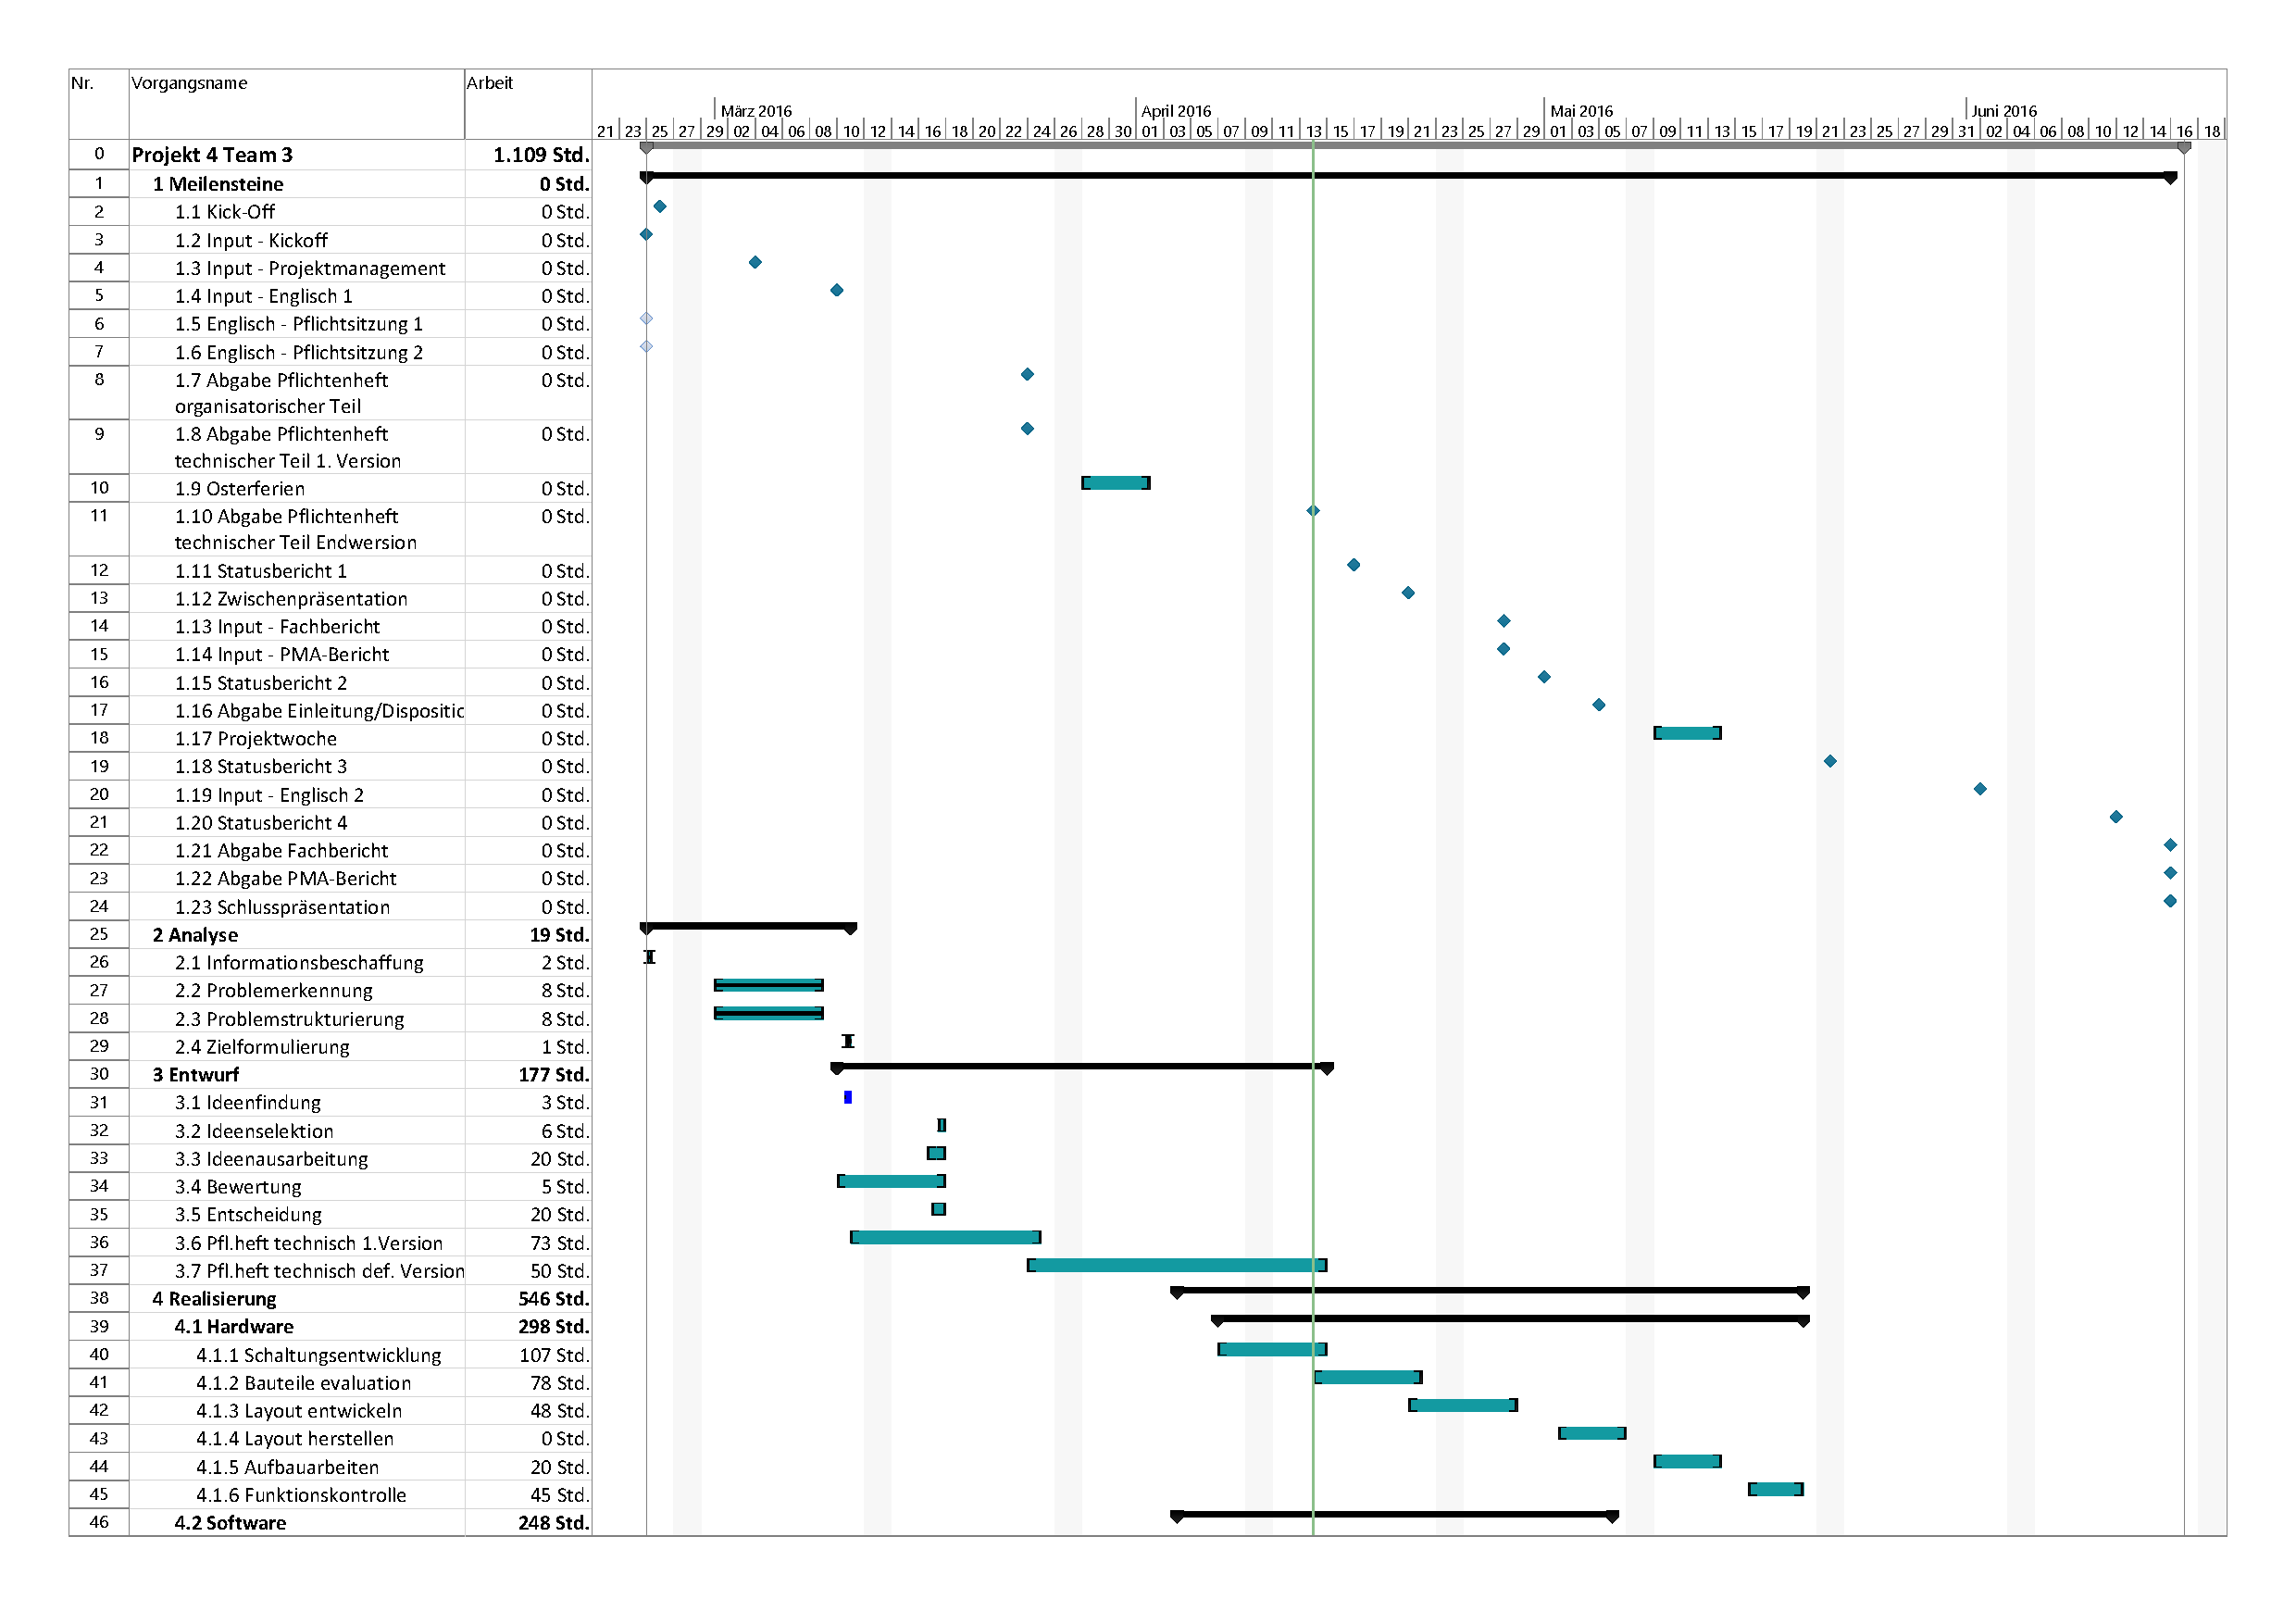
\includegraphics[width=1.22\textwidth,clip=true,trim=0 20mm 0 13mm]{images/psp.pdf}
%    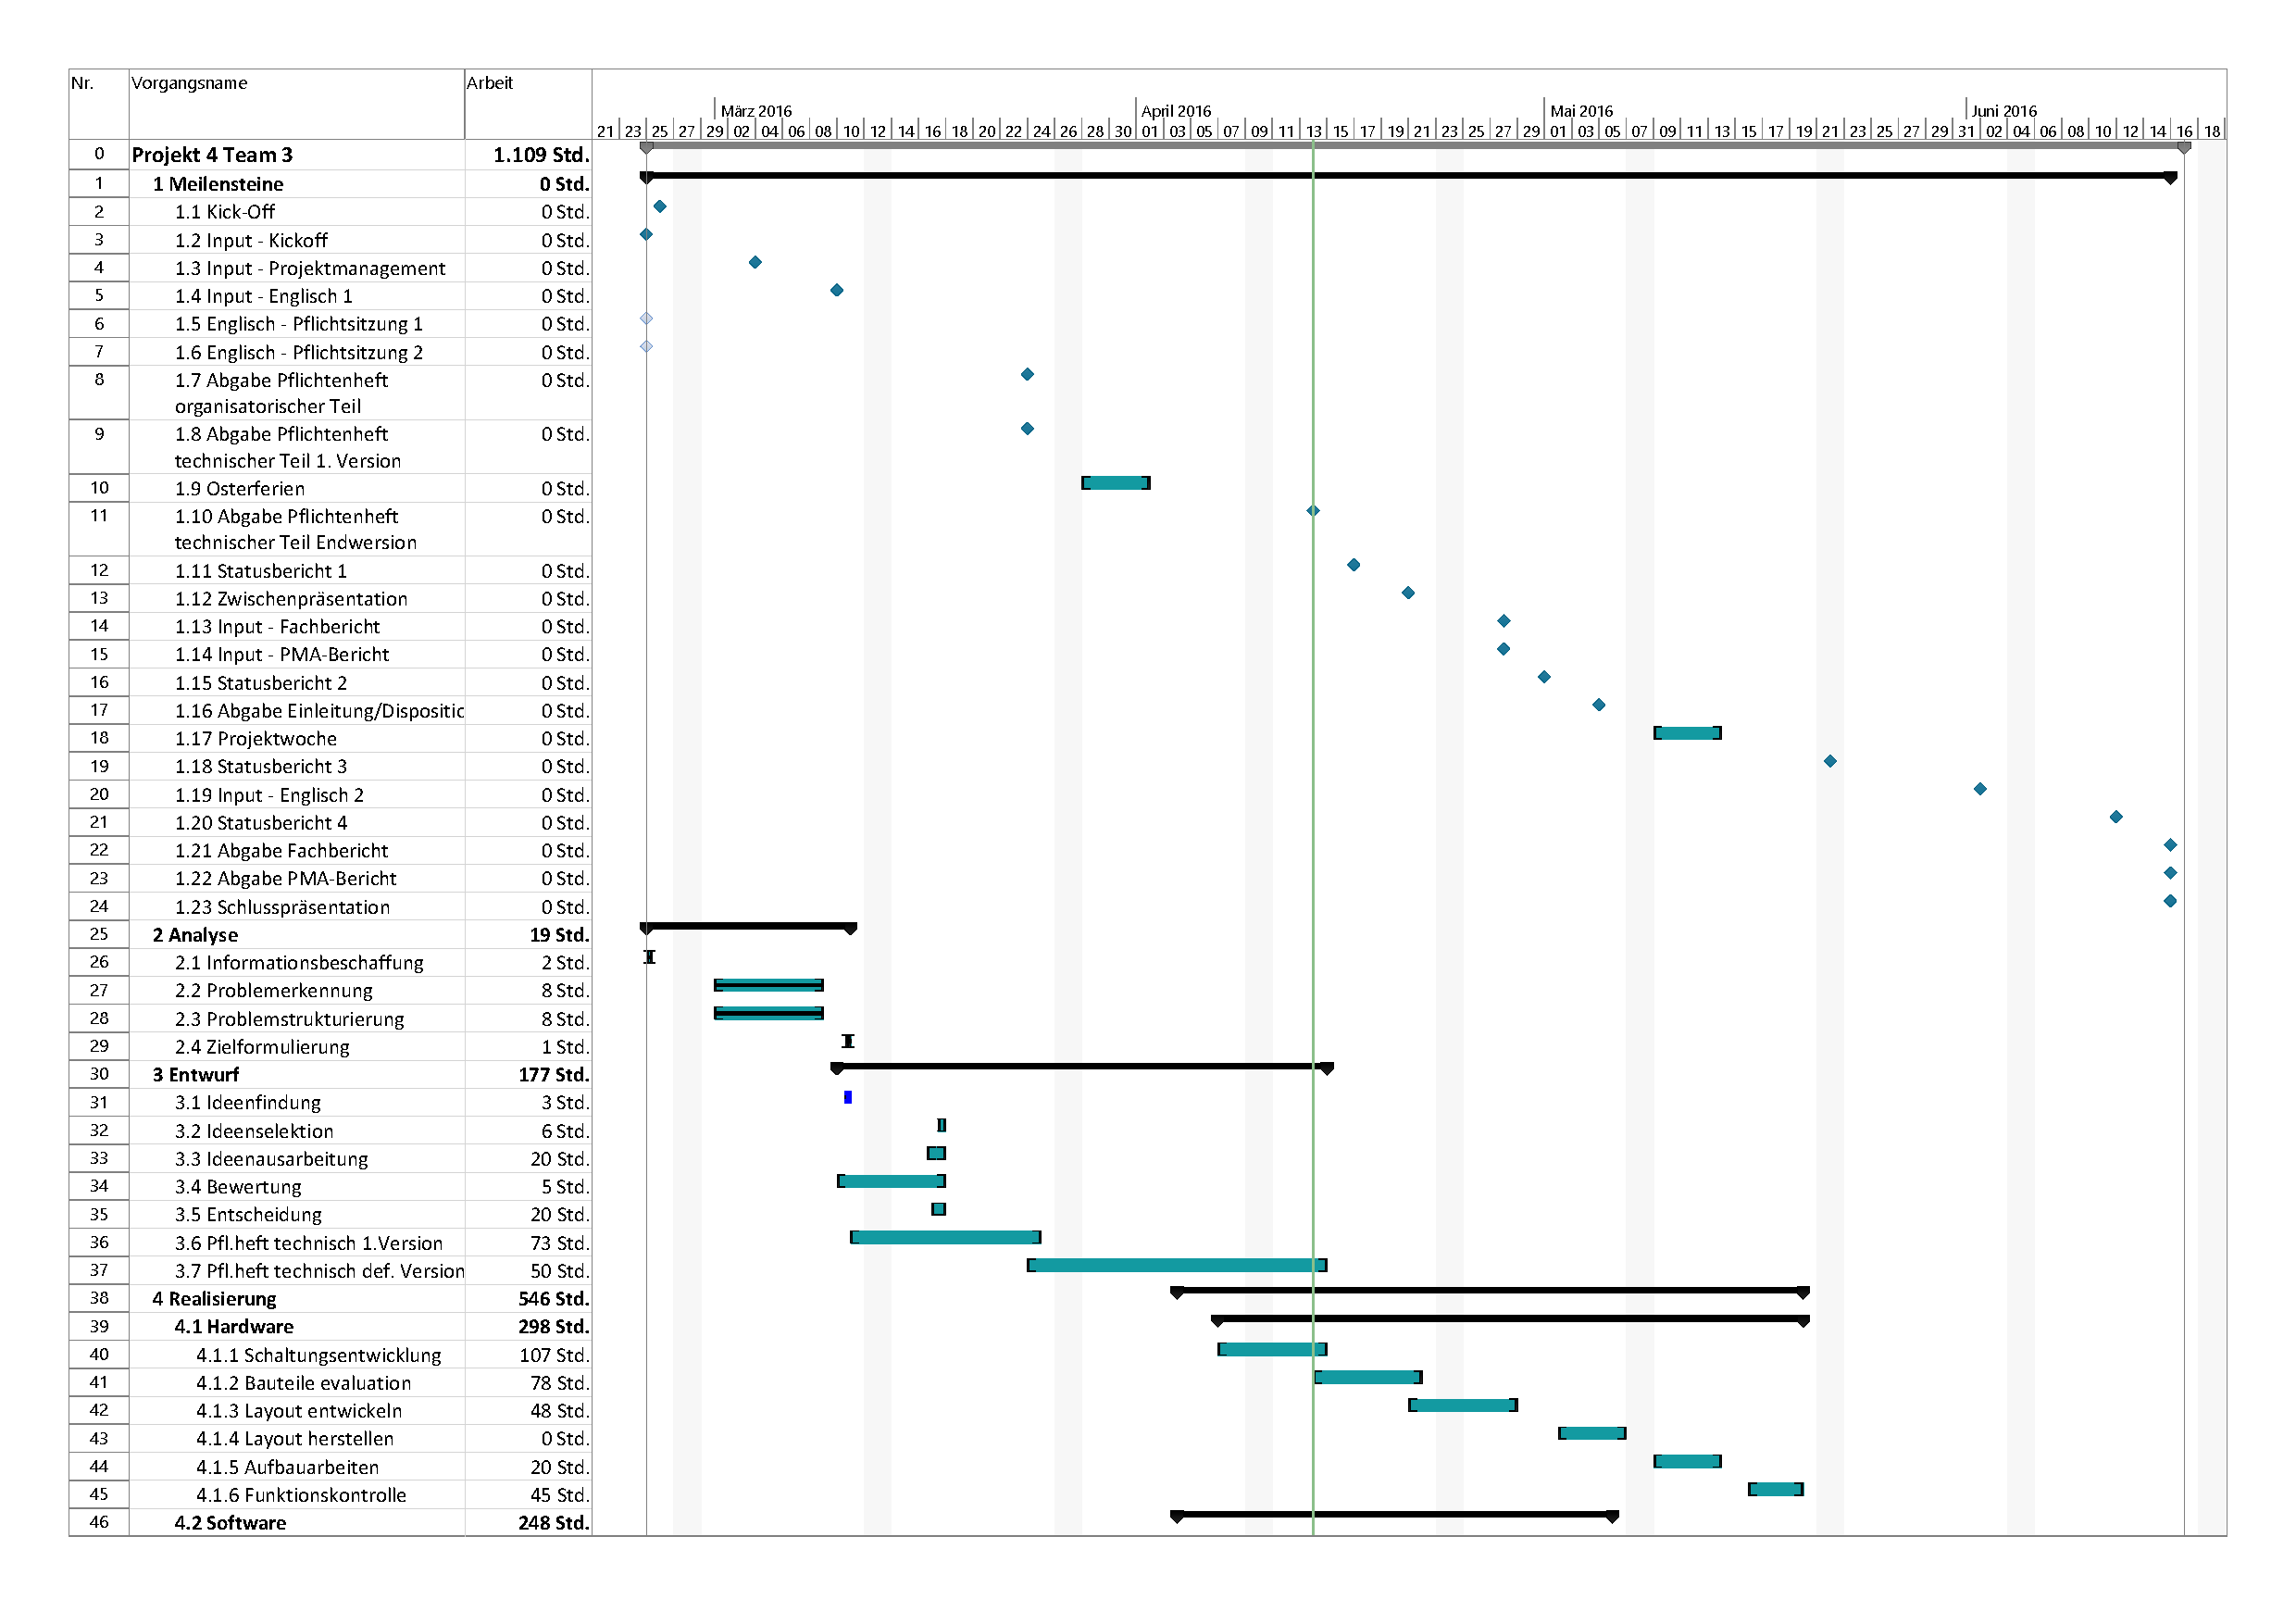
\includegraphics[width=.5\textwidth,clip=true,trim=0 0mm 0 0mm]{images/psp.pdf}
%    \caption{Projekstrukturplan und Personalterminplan, Kleinversion. Grossversion siehe Anhang \ref{appendix:zeitplan}}
%\end{center}
%\end{figure}

%\clearpage
%\setlength\paperheight{297mm}
%\setlength\paperwidth{420mm}
%\setlength\pdfpageheight{\paperheight}
%\setlength\pdfpagewidth{\paperwidth}
%
%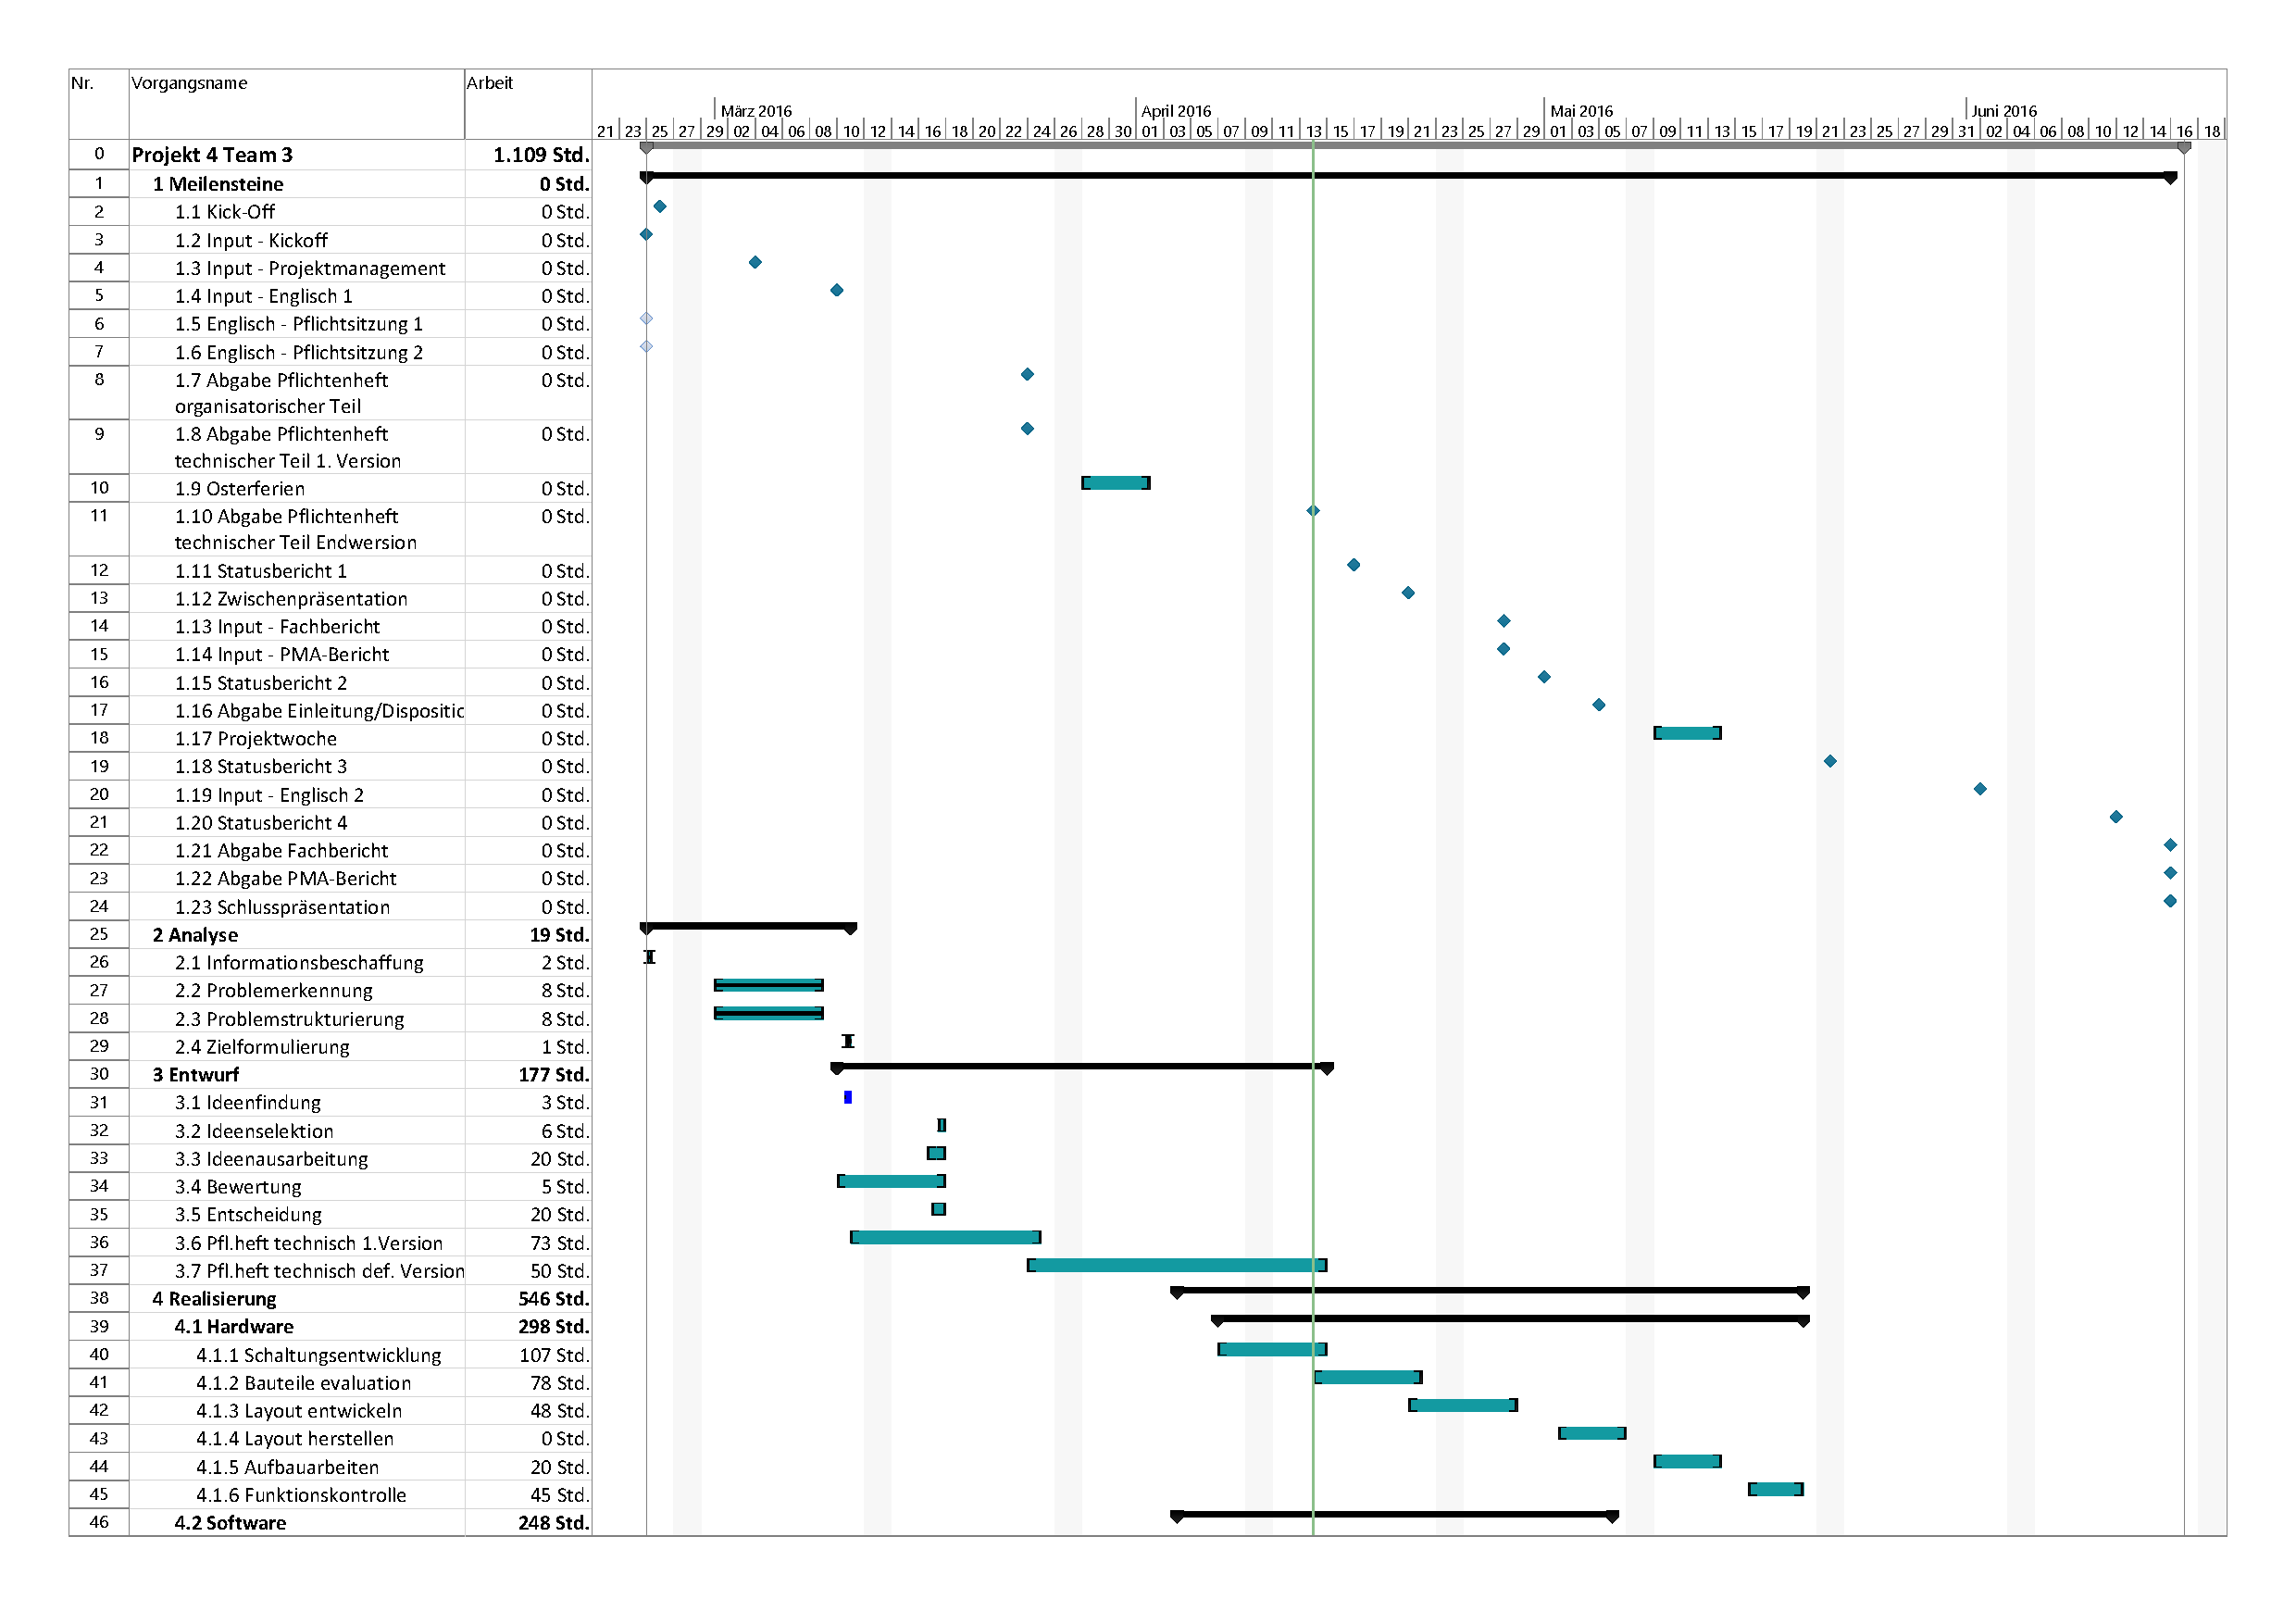
\includepdf[page=1-2,scale=1]{images/psp.pdf}
%
%\setlength\paperheight{297mm}
%\setlength\paperwidth{210mm}
%\setlength\pdfpageheight{\paperheight}
%\setlength\pdfpagewidth{\paperwidth}


%\vspace{30mm}
\begin{figure}[h!]
    \centering
    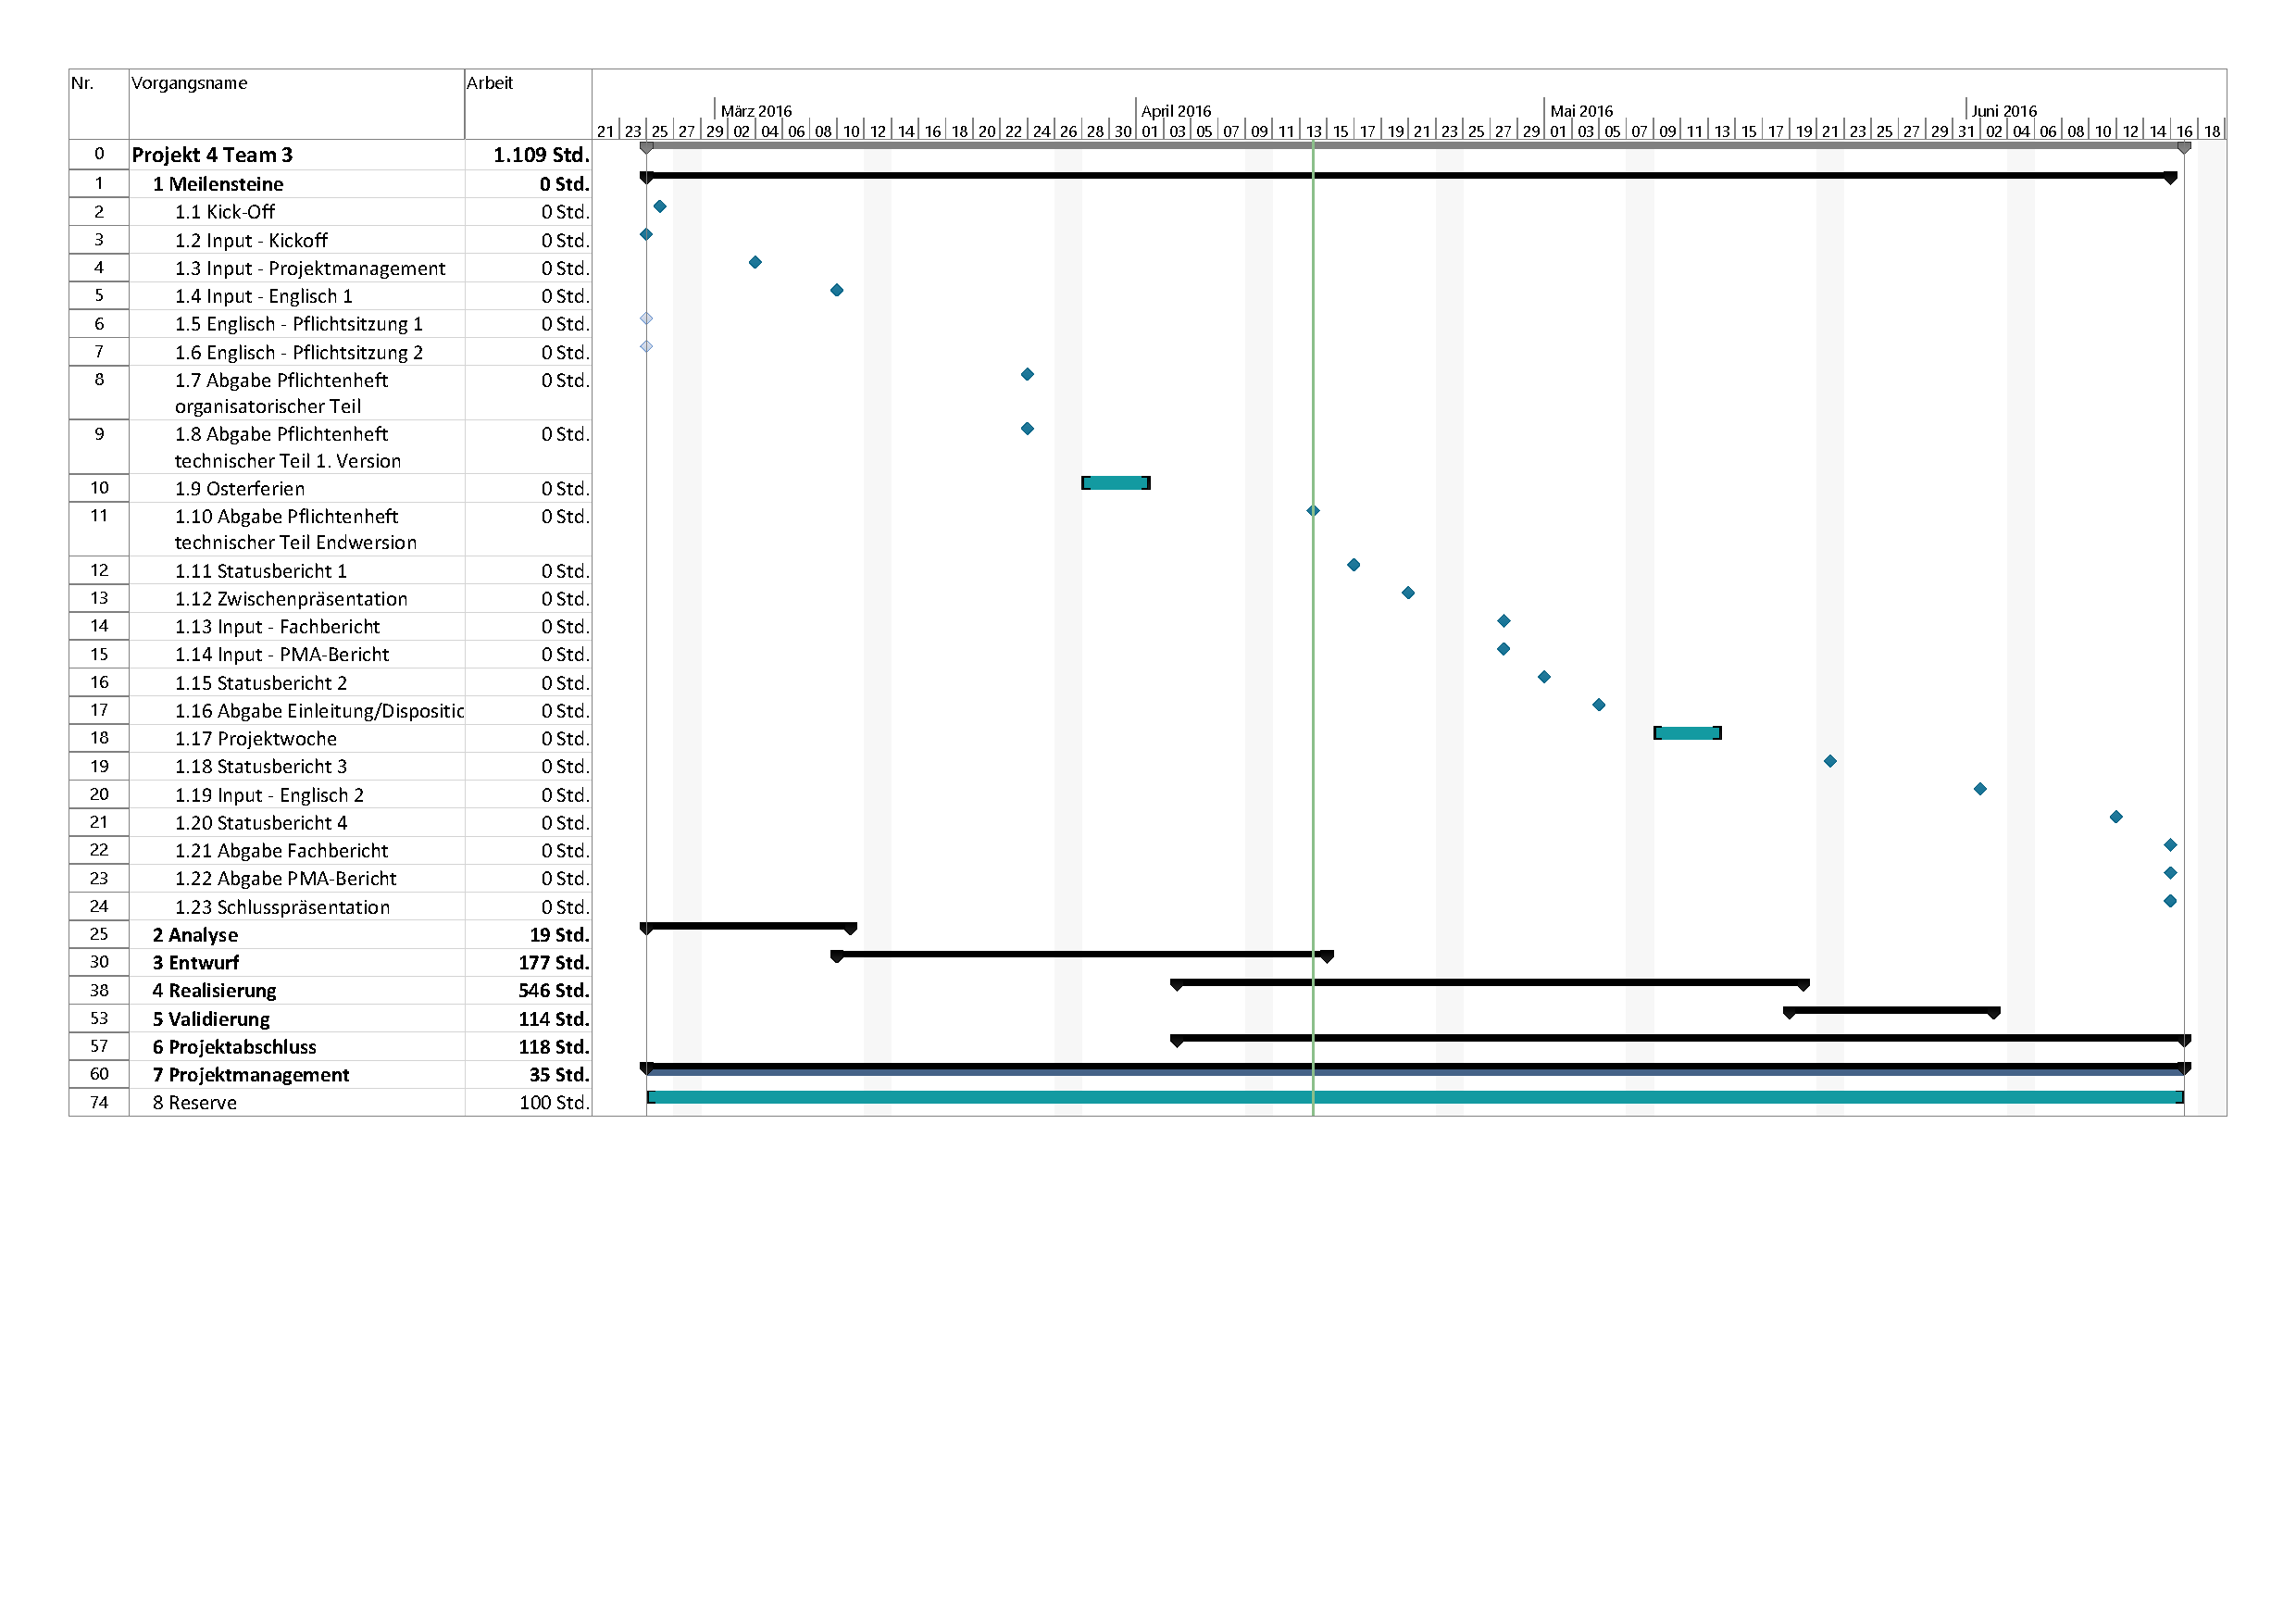
\includegraphics[width=1.55\textwidth,clip=true,trim = 10mm 80mm 0mm 0mm]{images/milestones.pdf}
    %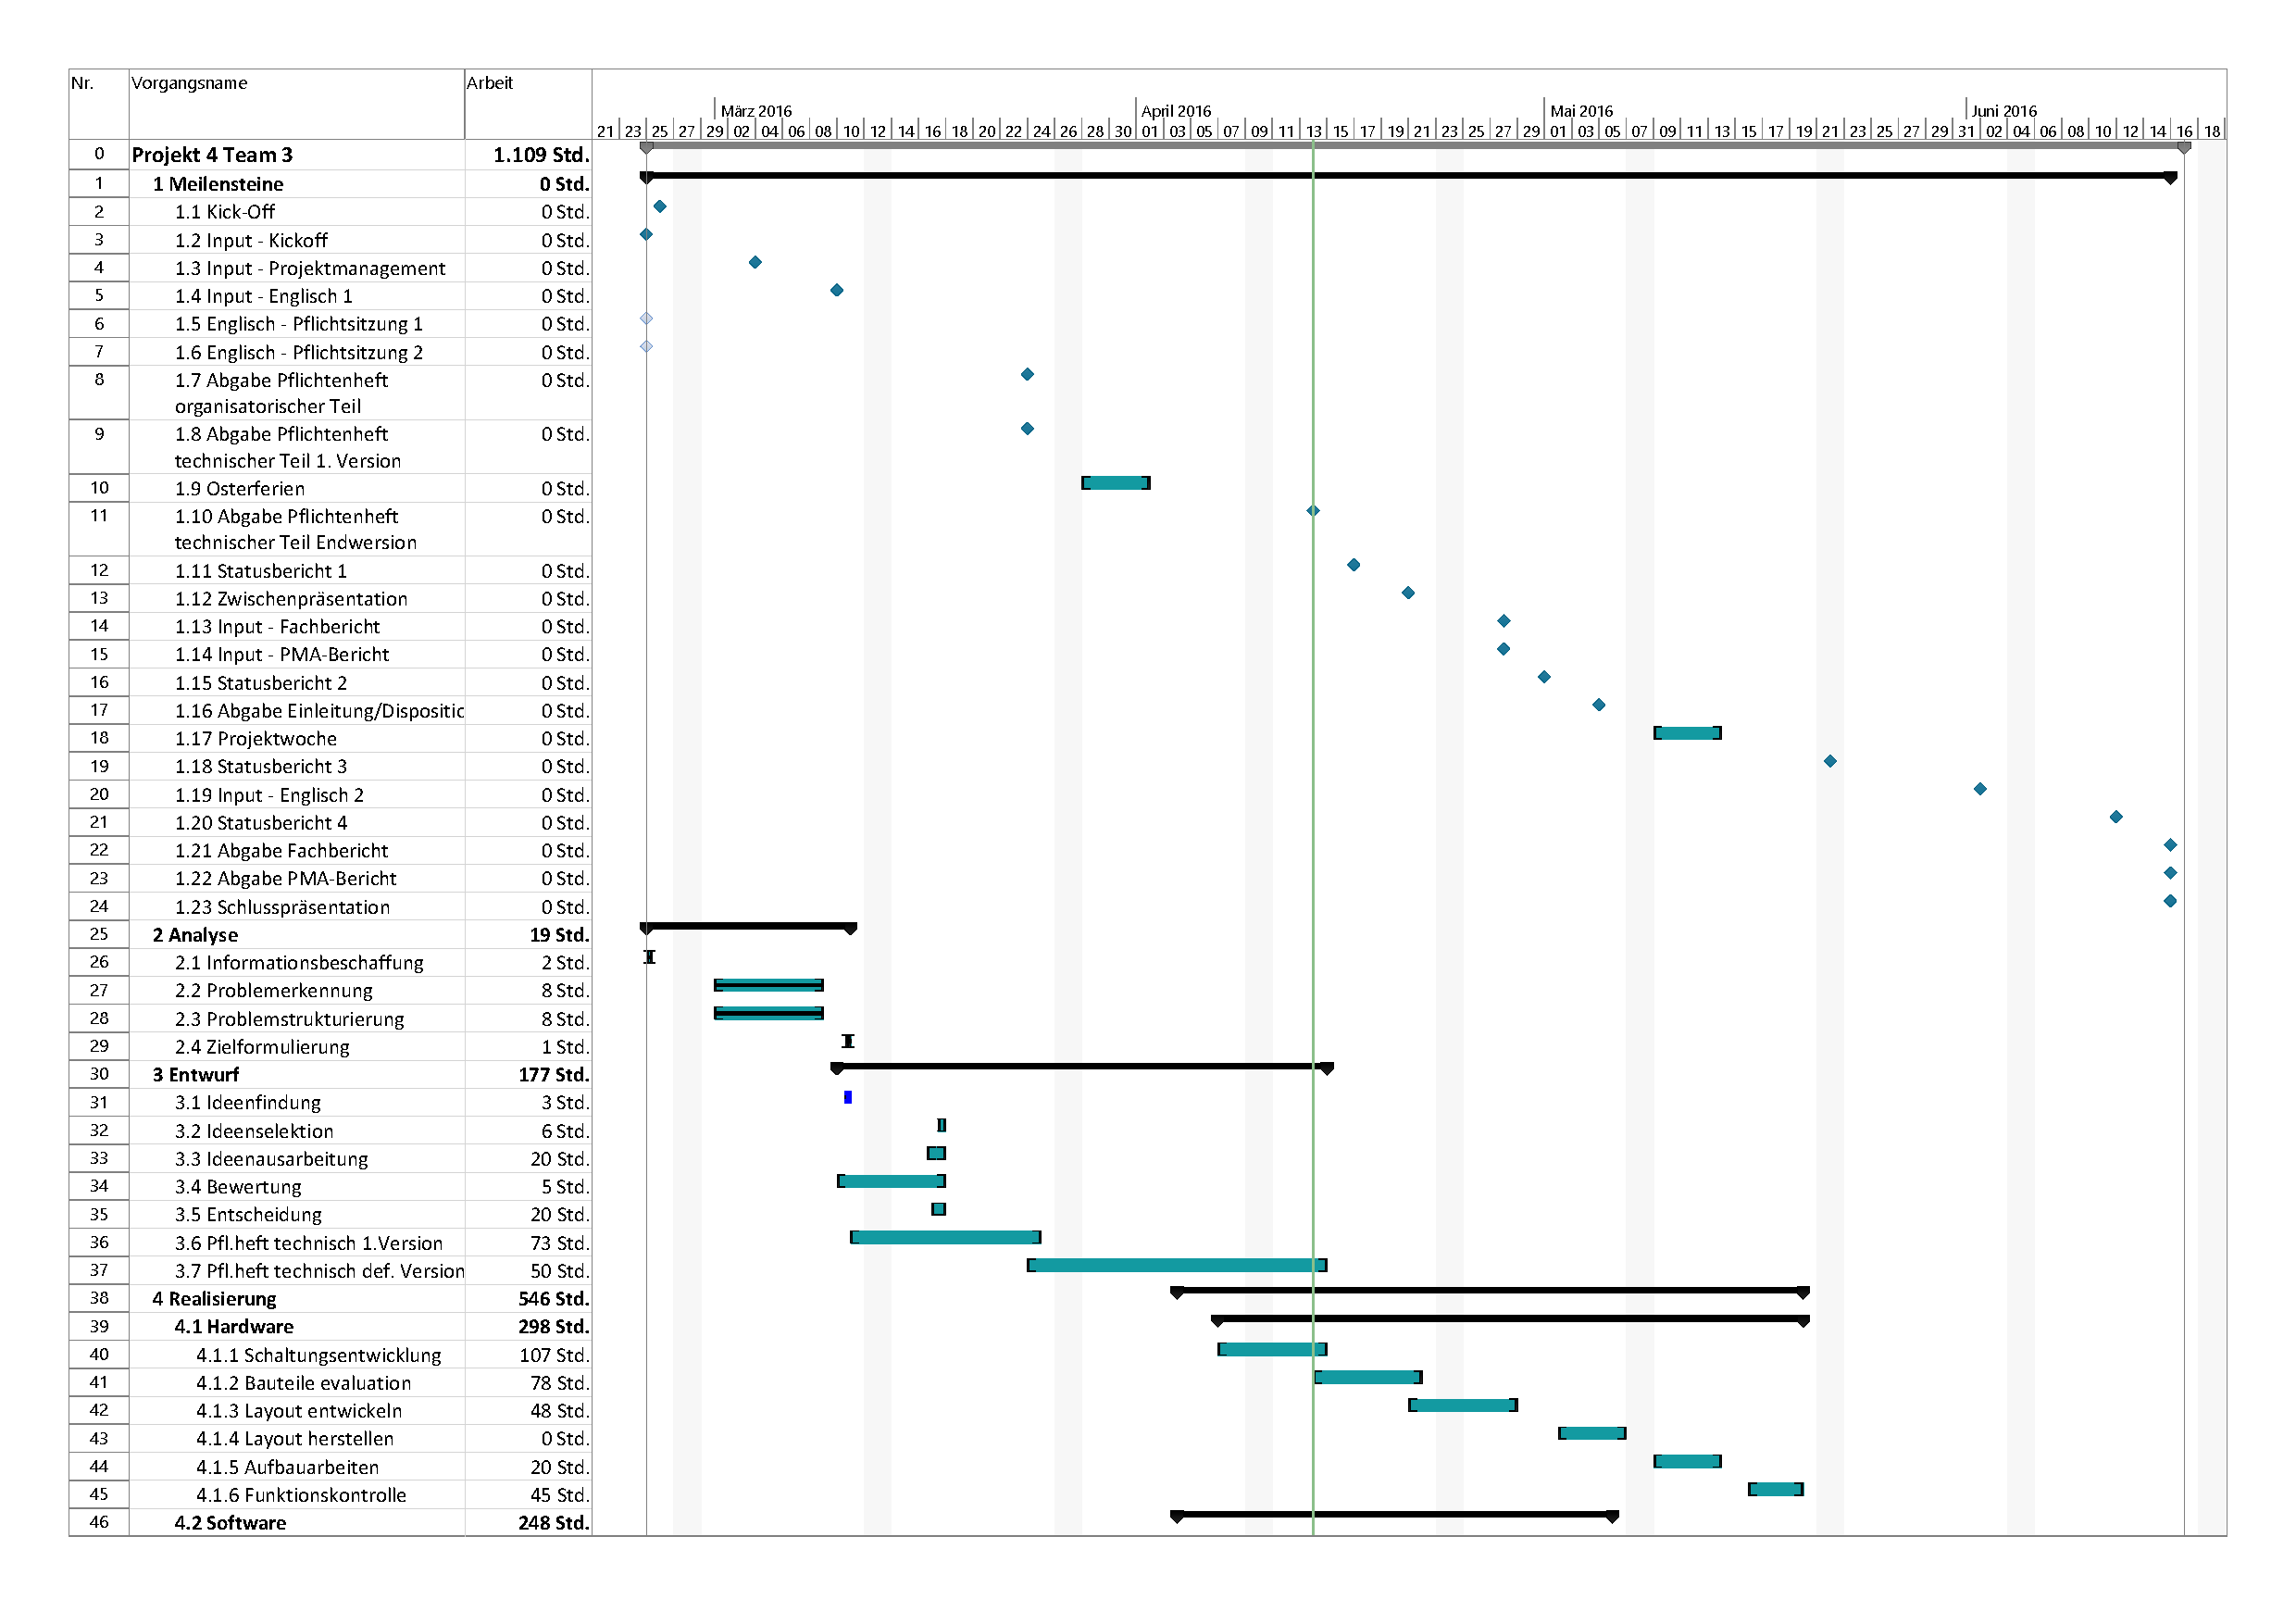
\includegraphics[width=.5\textwidth]{images/psp.pdf}
    \caption{Milestones}
    \label{fig:milestones}
\end{figure}
